\documentclass[a4paper,11pt]{article}
\usepackage{pgfplots}
\usepackage{siunitx}
\sisetup{detect-weight,exponent-product=\cdot,output-decimal-marker={,},
	per-mode=symbol,binary-units=true,range-phrase={-},range-units=single}
\SendSettingsToPgf
\usetikzlibrary{pgfplots.groupplots}
\pgfplotsset{compat=1.11}
\usepgfplotslibrary{external}
\tikzexternalize

\textwidth 160mm \textheight 247mm

\pgfplotsset{width=\figurewidth,compat=1.11}
\pgfplotsset{
	tick label style={font=\tiny},
	label style={font=\footnotesize},
	legend style={font=\footnotesize},
	title style={font=\footnotesize}
}


\newcommand{\szer}{16cm}
\newcommand{\wys}{5.6cm}
\newcommand{\odstepionowy}{1.2cm}


\begin{document}

\tikzsetnextfilename{}

\begin{figure}[Odpowiedź toru u1 - y1]
\tikzsetnextfilename{zad2_u1y1}
\begin{tikzpicture}
\begin{groupplot}[group style={group size=1 by 2,vertical sep=\odstepionowy},
width=\szer,height=\wys]
%%1
\nextgroupplot
[xmin=1,xmax=400,ymin=30,ymax=50,
xtick={0,50,...,800},
ytick={0,5,...,100},
ylabel={$T_1(t)$},
xlabel={$t$}]
\addplot[const plot,color=blue,semithick] file {datadir/T1_G1_39.txt};
\addplot[const plot,color=red,semithick] file {datadir/T1_G1_49.txt};
\addplot[const plot,color=green,semithick] file {datadir/T1_G1_69.txt};
\legend{$G1 = 39$,$G1 = 49$,$G1 = 69$}
\end{groupplot}
\end{tikzpicture}
\end{figure}

\begin{figure}[Odpowiedź skokowa toru u1 - y2]
\tikzsetnextfilename{zad2_u1y2}
\begin{tikzpicture}
\begin{groupplot}[group style={group size=1 by 2,vertical sep=\odstepionowy},
width=\szer,height=\wys]
%%1
\nextgroupplot
[xmin=1,xmax=400,ymin=30,ymax=50,
xtick={0,50,...,800},
ytick={0,5,...,100},
ylabel={$T_2(t)$},
xlabel={$t$}]
\addplot[const plot,color=blue,semithick] file {datadir/T2_G1_39.txt};
\addplot[const plot,color=red,semithick] file {datadir/T2_G1_39.txt};
\addplot[const plot,color=green,semithick] file {datadir/T2_G1_39.txt};
\legend{$G1 = 39$,$G1 = 49$,$G1 = 69$}
\end{groupplot}
\end{tikzpicture}
\end{figure}


\begin{figure}[Odpowiedź skokowa toru u2 - y1]
\tikzsetnextfilename{zad2_u2y1}
\begin{tikzpicture}
\begin{groupplot}[group style={group size=1 by 2,vertical sep=\odstepionowy},
width=\szer,height=\wys]
%%1
\nextgroupplot
[xmin=1,xmax=400,ymin=30,ymax=50,
xtick={0,50,...,800},
ytick={0,5,...,100},
ylabel={$T_1(t)$},
xlabel={$t$}]
\addplot[const plot,color=blue,semithick] file {datadir/T1_G2_44.txt};
\addplot[const plot,color=red,semithick] file {datadir/T1_G2_54.txt};
\addplot[const plot,color=green,semithick] file {datadir/T1_G2_74.txt};
\legend{$G2 = 44$,$G2 = 54$,$G2 = 74$}
\end{groupplot}
\end{tikzpicture}
\end{figure}

\begin{figure}[Odpowiedź skokowa toru u2 - y2]
\tikzsetnextfilename{zad2_u2y2}
\begin{tikzpicture}
\begin{groupplot}[group style={group size=1 by 2,vertical sep=\odstepionowy},
width=\szer,height=\wys]
%%1
\nextgroupplot
[xmin=1,xmax=400,ymin=30,ymax=50,
xtick={0,50,...,800},
ytick={0,5,...,100},
ylabel={$T_2(t)$},
xlabel={$t$}]
\addplot[const plot,color=blue,semithick] file {datadir/T2_G2_44.txt};
\addplot[const plot,color=red,semithick] file {datadir/T2_G2_54.txt};
\addplot[const plot,color=green,semithick] file {datadir/T2_G2_74.txt};
\legend{$G2 = 44$,$G2 = 54$,$G2 = 74$}
\end{groupplot}
\end{tikzpicture}
\end{figure}


\begin{figure}[Charakterystyka statyczna]
\tikzsetnextfilename{zad2_charstat}
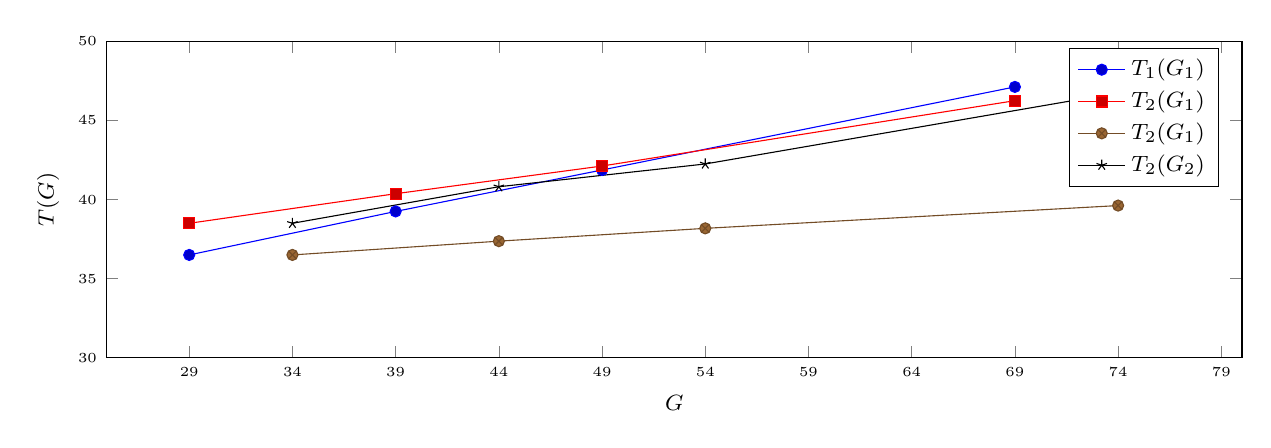
\begin{tikzpicture}
\begin{groupplot}[group style={group size=1 by 2,vertical sep=\odstepionowy},
width=\szer,height=\wys]
%%1
\nextgroupplot
[xmin=25,xmax=80,ymin=30,ymax=50,
xtick={4,9,...,800},
ytick={0,5,...,100},
ylabel={$T(G)$},
xlabel={$G$}]
    \addplot coordinates { (29,36.50000) (39,39.250000) (49,41.870000) (69,47.120000) }; 
    \addplot coordinates { (29,38.50000) (39,40.370000) (49,42.120000) (69,46.250000) }; 
    \addplot coordinates { (34,36.50000) (44,37.370000) (54,38.180000) (74,39.620000) }; 
    \addplot coordinates { (34,38.50000) (44,40.810000) (54,42.250000) (74,46.750000) }; 
	\legend{ $T_1(G_1)$, $T_2(G_1)$, $T_2(G_1)$, $T_2(G_2)$ }
\end{groupplot}
\end{tikzpicture}
\end{figure}

\end{document}
